\documentclass[12pt,fleqn]{article}
\setlength{\parindent}{0pt}
\usepackage{graphicx}
\usepackage{listings}
\usepackage[latin5]{inputenc}
\setlength{\parskip}{8pt}
\setlength{\parsep}{0pt}
\setlength{\headsep}{0pt}
\setlength{\topskip}{0pt}
\setlength{\topmargin}{0pt}
\setlength{\topsep}{0pt}
\setlength{\partopsep}{0pt}
\setlength{\mathindent}{0cm}

\begin{document}
Ders 3

Konumuz $Au = b$ sistemini cozmek. Bu cozum icin Python'da
\verb!linalg.solve! cagrisi var. Mesela

\lstinputlisting[language=Python]{solve1.py}

\verb!linalg.solve! cagrisi Matlab'de \verb!\! cagrisinin karsiligi,
oradaki kullanim u = A \verb!\! b seklinde. 

Eger elimizde ikinci bir \verb!c! vektoru var ise, ve esitligin sag
tarafinda \verb!b! sonrasi onu kullanmak istiyorsak ayri ayri \verb!solve!
komutlarina gerek yoktur. Her iki vektoru birbirine ekleyerek,
\verb!solve!'u toplu halde cagirabiliriz, bu performans acisindan daha iyi
olur. 

\begin{lstlisting}[language=Python]
c = [2,3,8]
bc = np.vstack((b,c)).T
u = scipy.linalg.solve(A,  bc)
\end{lstlisting}

Python \verb!vstack! komutu iki matrisi ust uste koymak icin kullanilir.

Her iki cozum beraber olarak geri gelecektir. Bu niye daha hizli? Cunku
Python'un cozucusu daha esitligin sag tarafina bile gelmeden sadece
\verb!A!'ya bakarak bir suru islem gerceklestiriyor, eliminasyon yaparak
\verb!A!'yi ucgensel hale getirmek gibi. Bu tur islemleri gereksiz kere iki
kere yapmak pahali olurdu.

Soru: matematiksel olarak $u$'yu bulmak 

\[ Au = b \]

\[ u = A^{-1}b \]

demektir. Peki Python bu hesap icin gercekten $A^{-1}$'i hesaplar mi?

Hayir. Cunku buyuk problemler icin matris tersini hesaplamak oldukca
pahalidir. Ayrica $A$ matrisi zaten ucgensel capraz (tridiagonal) bir halde
olabilir, ve cevap zaten hazir haldedir, bu noktada ters alma islemi
gereksiz olurdu. 

Biraz zihin egzersizi yapalim. Eger soyle bir komut kullansam ne elde
ederim (ki \verb!I! matrisi birim matrisi) ?

\begin{lstlisting}[language=Python]
solve(A, I)
\end{lstlisting}

Cevap, tabii ki $A$'nin tersini elde ederim, yani $A^{-1}$ cunku $AA^{-1} =
I$, 
sag tarafta birim matrisi var ise cozum sadece $A^{-1}$ olabilir.

\[ 
A 
\left[\begin{array}{rrr}
u_1 & u_2 & u_3
\end{array}\right]
=
\left[\begin{array}{rrr}
1 & 0 & 0\\
0 & 1 & 0\\
0 & 0 & 1
\end{array}\right]
 \]

Bu probleme bakmanin degisik bir yolu: sag taraftaki birim matrisi icindeki
[1 0 0] gibi degerler icindeki 1 degerlerini birer ziplama (impulse) ani
gibi gormek, sanki elimizde bir duz [0 0 .. 0] bir veri var, icinde tek
ziplama olan yer orasi, ve bu [1 0 0], [0 1 0], .. icinde tek ziplama olan
veriler ``islenerek'' bize $u_1$, $u_2$, .. gibi sonuclari veriyorlar. 

Elle $A$'nin tersini bulmak icin ne yapardik? Bir blok matrisi yaratirdik,
\verb![A I]!, yani 3x3 ve 3x3 iki matrisi yanyana koyup 3x6 boyutunda yeni
bir matris elde ederdik, ve bu matriste $A$ uzerinde eliminasyon, pivotlari
sifirlama gibi numaralari kullanarak onu birim matrise cevirirdik, bu arada
ayni operasyonlari tabii ki $I$ uzerinde uygulardik. En sonunda $A$ birim
olunca $I$ $A^{-1}$'e donusmus olurdu!

Simdi biraz buyuk resme bakalim. 

Lineer cebirin 4 buyuk problemi Python komutlari ile beraber sunlardir:

Eliminasyon, 
\verb!scipy.linalg.lu(A)! $A = LU$

Dikeylestirme / ortogonalastirma (orthogonalization), 
\verb!scipy.linalg.qr(A)!, $A = QR$

Ozdegerler (eigenvalues), 
\verb!scipy.linalg.eig(A)! $A = SAS^{-1}$

Tekil degerler (singular values), 
\verb!scipy.linalg.svd(A)! $A = U \Sigma V^{T}$

Eliminasyon ne yapar? Dikkat edersek aslinda bu islemin bir alt ucgensel
(lower triangular) matris ($L$) ve bir tane de ust ucgensel matris ($U$)
ortaya cikardigini goruruz. Simdi alttaki matris uzerinde eliminasyon
yapalim ve bu arada tersini de bulmus olalim. 

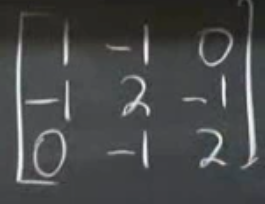
\includegraphics[height=2cm]{3_2.png}

Eliminasyon islemlerini yapalim. 

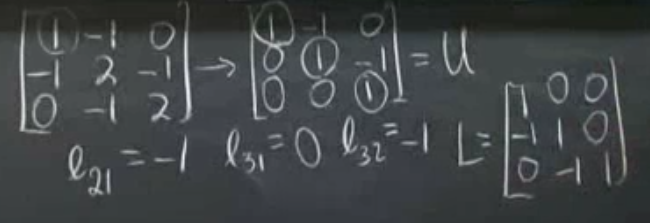
\includegraphics[height=2cm]{3_3.png}

$l_{21} = -1$ yapilan ilk islemi kodluyor, 1. satiri -1 ile carp ve
2. satirdan cikart anlamina geliyor. Digerlerini de sirasiyle goruyoruz ve
bu islemlerin sonucunda ust ucgensel matris $U$'yu elde ediyoruz. Tum $l$
degerlerini bir araya koyup $L$'yi elde edebiliriz. Bir tane daha yapalim:

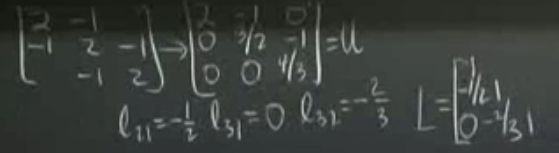
\includegraphics[height=2cm]{3_4.png}

Eger tekil (singular) bir matris uzerinde eliminasyon yapsak, bu islemi
nasil etkilerdi? 

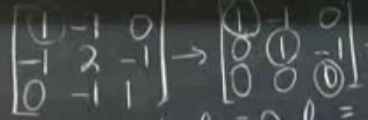
\includegraphics[height=2cm]{3_5.png}

Yani bu durumda 3 tane pivot elde edemezdik, sag alt kosedeki deger
eliminasyon sirasinda 0 olurdu, ve sag matris, aynen sol matris gibi, tekil
olurdu. Bu isimize yaramazdi. 

Su probleme donelim: 

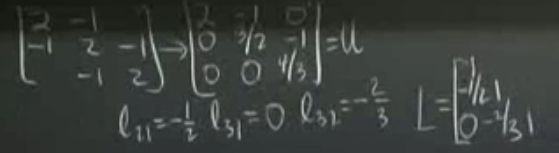
\includegraphics[height=3cm]{3_4.png}

Burada ilk matris simetrik idi, ama $L$ ve $U$ matrisi artik simetrik
degil. Simetriyi geri getirebilir miyiz? $U$ icinden sadece caprazlari
cekip cikartalim

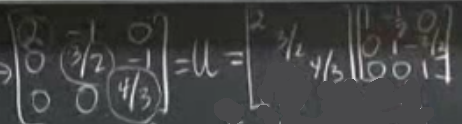
\includegraphics[height=3cm]{3_6.png}

Boylece caprazinda [2 3/2 4/3] olan bir matris elde ettik. Peki bu matrisin
carptigi (onun hemen saginda) icinden caprazlari cekip cikardigimiz
matristen geri kalanlar tanidik geliyor mu? Evet, bu matris te $L^T$'e
esit. Demek ki $LU = LDL^T$ gibi bir ifade mumkun.

Biliyoruz ki 

$K = LDL^T$

ifadesinde $K$ her zaman simetriktir. Ters yonden soylersek, herhangi bir
simetrik $K$ matrisini alip eliminasyon yaparsam ve $L$ ve $D$ elde edince,
$L^T$ ile carpabilirim. 

Peki sunu ispat edebilir miyiz? Herhangi bir $L$ ve capraz $D$ var ise,
$LDL^T$ her zaman simetrik midir? Bir matrisin simetrik olmasi demek
kendi devrigine (transpose) esit olmasi demektir. Yani 

\[ K = LDL^T \]

\[ K^T = (LDL^T)^T \]

Devrigi alinca parantez icindeki carpimlarin sirasi degisir.

\[ = (L^T)^TD^TL^T \]

$D^T = D$ cunku $D$ zaten capraz bir matris, onemli tum degerleri
caprazinda ve devrik islemi bu durumu degistirmiyor. O zaman

\[ = LDL^T \]

Tekrar basladigimiz noktaya donduk. Demek ki basladigimiz matris
simetriktir. Ispat tamamlandi. 

Genele donelim: $A^TA$'nin mesela karesel oldugunu biliyorduk (nxm ile mxn
carpilinca nxn boyutu elde edilir). Simdi bunun uzerine simetrik oldugunu
da artik biliyoruz, ustte ispatladik.

Kural: Simetrik matrislerin tersi (inverse) de simetriktir. O zaman
$K^{-1}$ de simetriktir. 

\end{document}







